\chapter{Literature Review}
\label{ch:lit-review}

The literature review is broken into five sections.  I first examine
what a season \emph{is}; how they are defined and why this matters.
I then explain tropical seasonality as understood by climate scientists,
before giving an academic perspective on Indigenous Knowledge.
I cover the literature on Indigenous seasons with a particular
focus on Northern Australia, and finally identify a broad gap in the
literature which this thesis begins to fill.

\todo{This whole chapter still needs work.}
\todo{revise opening after draft completed.}

~\\

\todo{
Justify the importance of seasons and this research.
Link research in historical climate change somewhere.
Have strong link between Indigenous seasons and phenology --
look for IweatherK too, BOM site?
}



\section{The Tropical Climate}
\label{sec:lit-tropical-climate}
\todo{write this section}


\todo{
Tropical seasonality, including monsoon and ENSO -- lays out simple scientific view.
(REFS - \citet{cook2001}, \citet{holland1985}).
%
Need to cover why seasons matter (reinforcing introduction);
should tie closely into section on tropical climatology
%
Looking at onset issue - in the tropics in Africa, the ITCZ move
is very marked; literature in Tanzania and Keyya has a double wet
seasons, as it goes north and south.  Very distinctive.
Sharron Nickleson at U Florida State, 80s and 90s
%
I.J. Clim. has references.  Not Indig, but very interesting,
looking at pure fluid climatology.
}\\



Tropical climates and seasons are driven by three global patterns of
atmospheric circulation:  Hadley cells, the coriolis effect, and the axial
tilt of the earth.

\begin{wrapfigure}{r}{0.6\textwidth}
    \centering
    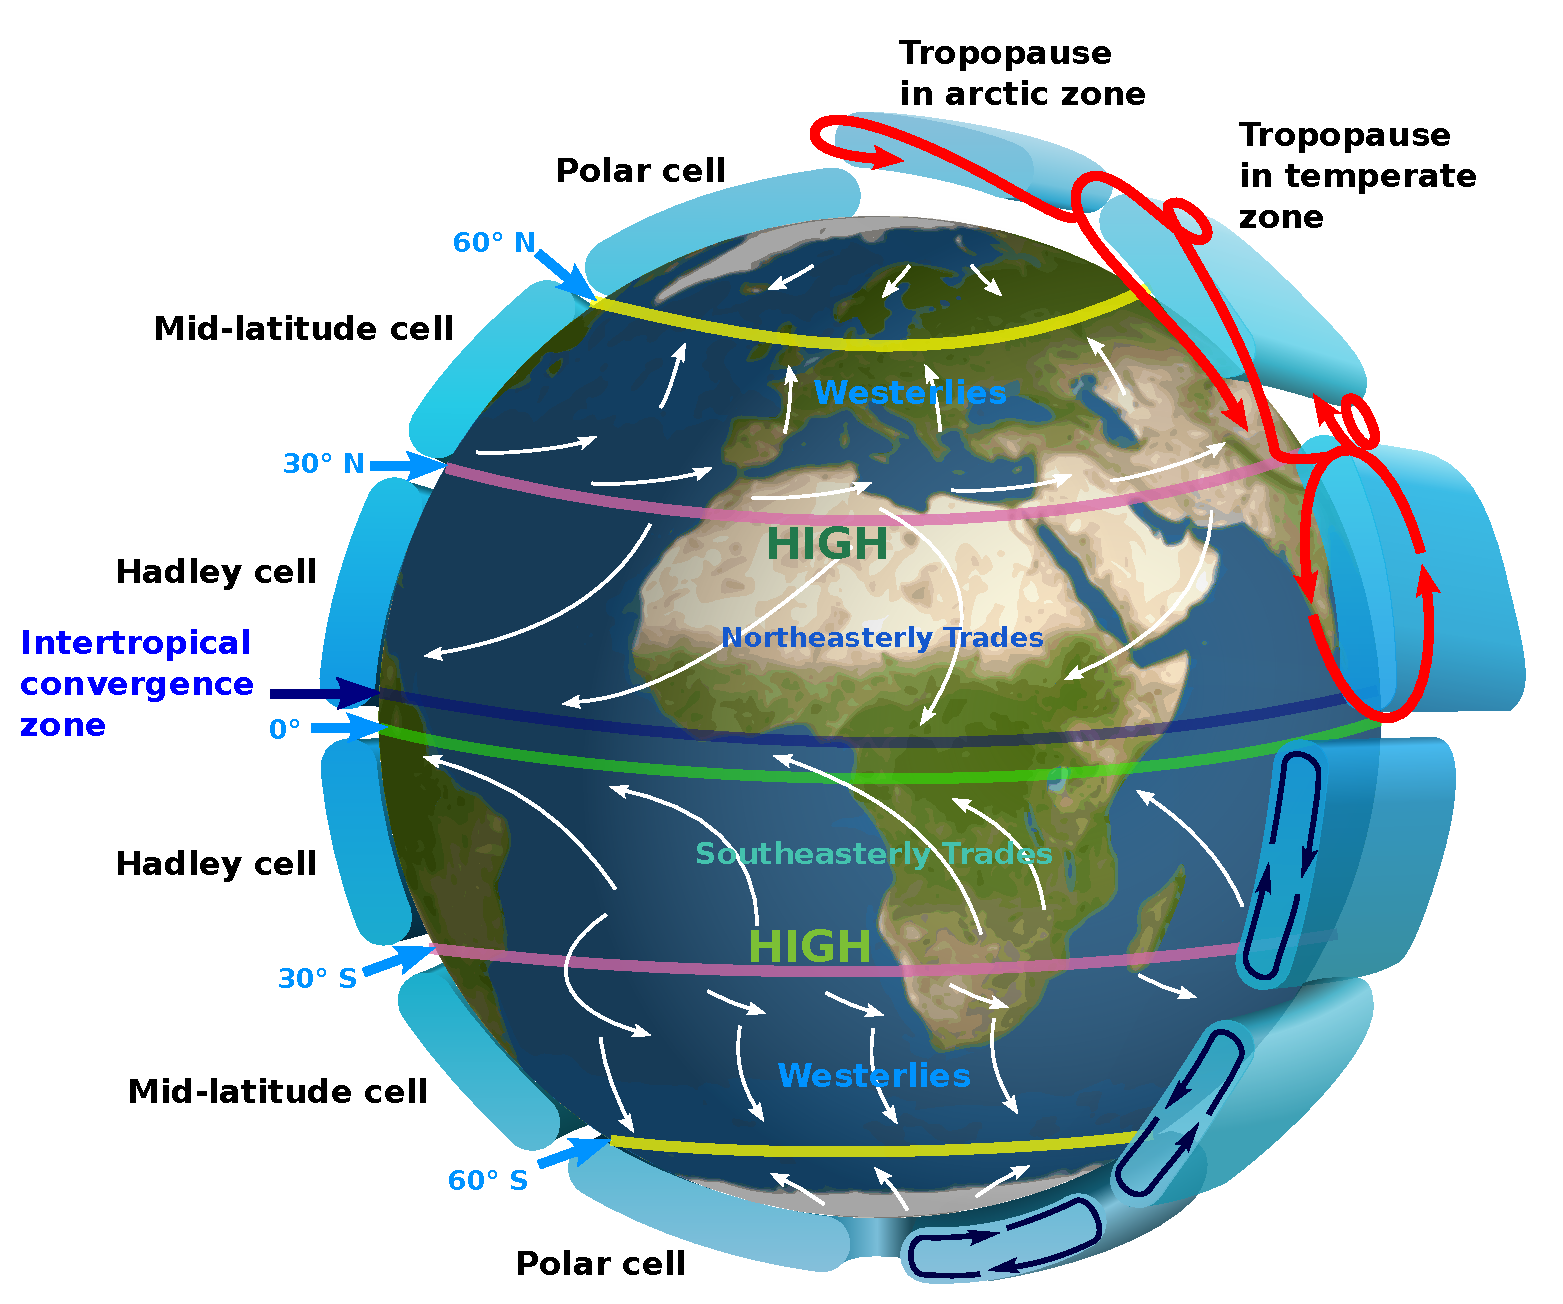
\includegraphics[width=\linewidth]{Earth_Global_Circulation.pdf}
    \caption[Hadley Cells and trade-winds]{
        Simple diagram showing surface-level prevailing winds (white arrows),
        Hadley Cells, and the Intertropical convergence zone (`ITCZ').
        Air rises at the ITCZ, heated by the highest - intensity sunlight.
        This causes a low-pressure band of trpoical rainfall, and the
        trade winds -- deflected towards the west by the Coriolis Effect.
        (image: Wikipedia)}
    \label{fig:hadley-cells}
\end{wrapfigure}

Hadley cells are a feature of the global atmospheric circulation
caused by the change in insolation -- solar energy delivered per area --
with latitude.  Insolation is greatest at the equator, and the hot air drops
rain as it rises and cools, then spreads towards the poles at high altitude.
At the surface, air tends to move towards the \textit{inter-tropical
convergence zone} (ITCZ), causing the trade winds and distinctive wet band
of the tropics.  The mid-latitude and polar cells shape climates at higher
latitudes, but are not directly relevant to tropical seasonality.

Monsoon seasonality can be understood as the ITCZ moving north or south,
following the latitude of greatest insolation -- which changes due to the
axial tilt of the Earth as it orbits the sun.  While this is strongly
associated with rainfall, the fundamental indicator is the direction of
the prevailing wind: generally south-easterly below the ITCZ, and generally
north-westerly above.  \Cref{fig:itcz-india-aus} shows how this pattern
manifests in reversed seasons between India and Northern Australia.

\begin{figure}[h]
    \centering
    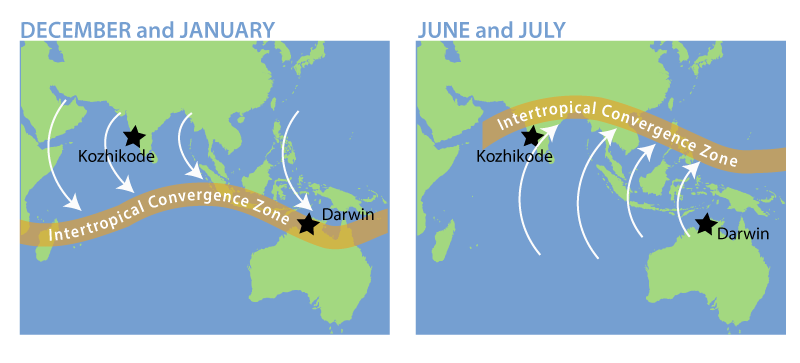
\includegraphics[width=0.8\linewidth]{itcz.png}
    \caption[ITCZ showing northern and southern monsoon]{
        Approximate location of the inter-tropical convergence zone
        (yellow band) during the northern and southern monsoon.
        White arrows show prevailing wind direction; rainfall is
        associated with the ITCZ.  \citep[image:][]{boos2014}}
    \label{fig:itcz-india-aus}
\end{figure}

~\\


At a more local scale, a monsoonal cycle is often described with a `Wet'
and a `Dry' season; in the Northern Territory both are warm to hot but
the humidity (and wind direction) is highly distinctive.
%
\Cref{fig:galiwinku-climograph} shows a `climograph', summarising monthly
averages for temperature and rainfall for Galiwinku -- which exhibits the
characteristic pattern of tropical seasons with a distinct hot/wet and
cooler/dry season, with far less variation in temperature and higher
humidity than temperate seasons.
%
The more nuanced patterns described by Indigenous seasons are not visible
in this figure; \cref{ch:results} shows that that requires more variables
observed at daily resolution.

\begin{figure}[h]
    \centering
    \includegraphics[width=\linewidth]{galiwinku/climograph.pdf}
    \caption[Monthly Climograph for Galiwinku]{
        Monthly summary of climate statistics at Galiwinku, showing the per-day
        mean for each month.  Rainfall (vertical bars), maximum temperature
        (solid line), minimum temperature (dashed line), and  dewpoint
        temperature (dotted line).  Dewpoint temperature is a measure of humidity.}
    \label{fig:galiwinku-climograph}
\end{figure}




\section{Indigenous Knowledge}
\label{sec:lit-iek}
\todo{write this section}

There are a variety of terms used in the literature to describe Indigenous
ecological knowledge systems:  \citet{clarke2009} refers to `land-based knowledge',
\citet{petheram2010} and \citet{turner2009} use `traditional ecological
knowledge', while \citet{cochran2015} simply use `indigenous knowledge'.
\citet{berkes2012} defines Indigenous Ecological Knowledge (IEK) as ``a cumulative
body of knowledge, practice and belief, evolving by adaptive processes and
handed down through generations by cultural transmission''.  I prefer
`Indigenous knowledge' to emphasise that ecology is not the only subject of
Indigenous knowledge - for example, seasonal calendars often have cultural and
economic as well as ecological importance.

WHY IS THIS KNOWLEDGE IMPORTANT - expands to why my research matters.
(related to fine-scale timing, as the nuance matters in land and NRM)

There is a growing recognition among ecologists, natural resource managers, and
scholars worldwide that Indigenous peoples hold important knowledge about the
natural environment. The literature on IEK is well-established and vibrant.  In
Australia and around the world, the value of Indigenous knowledge is recognised
in areas as diverse as climate change and sustainability assessment
\citep[eg.][]{cochran2015}, holistic fire management \citep[eg.][]{clarke2009,price2012},
customary economic activities including aquaculture \citep{woodward2012a}, and
natural resource management \citep[eg.][]{prober2011}.  The \textit{Environment
Protection and Biodiversity Conservation Act 1999} suggests taking `a
partnership approach to environmental protection and biodiversity conservation'
\citep{ens2012}, which is increasingly common at local and state levels.

\citet{turner2009} distinguish Indigenous knowledge systems from `objective'
scientific knowledge on the basis that Indigenous knowledge of practical
matters is value-laden and observations or experience are tangled with beliefs,
philosophy, law, and spirituality.  \citet{green2010a} and \citet{clarke2009}
demonstrate the use of Indigenous phenological and climate knowledge to improve
western scientific understanding of past and future climates.
EXPAND THIS PARA, see also recent Woodward paper.

This literature provides a rich context for synthesis of indigenous knowledge
and western climate science to investigate Australian seasonality.
TO WHAT END?



\subsection{Two-ways research}
Broaden approach; not just two-ways - read other research methodology and
situate work.  Really really need to do this.

Around the world, and more recently in Australia, there has been growing
interest in `two-ways' research \citep{turner2009,prober2011},
which ``uses combinations of Indigenous and non-Indigenous knowledge and
methods, and with the involvement of both Indigenous and non-Indigenous people
towards a common goal'' \citep{ens2014}.

However, working across knowledge systems can be difficult for both Indigenous
and non-Indigenous people, and often challenges institutions and research
funding bodies to invest substantial time and resources in relationship-
building with uncertain outcomes.  The Ngan'gi Seasons Calendar emphasises
ecological events and customary activities for each season above the timing and
meteorological conditions.  Produced in collaboration between Ngan'gi knowledge
holders and the CSIRO, `success' required a long-term commitment to work in
remote areas on the Daly River, a high degree of risk tolerance in
research funding, and many years work building solid relationships \citep{woodward2010}.

\todo{A bit thin; expand benefits and value of knowledge}

When \citet{petheram2010} investigated perspectives on climate change
adaptation in NE Arnhem Land; the community engaged in terms of resilience to
existing issues rather than adaptation to climate change, challenging the basis
of their research.  With severe problems related to poor housing, drug abuse,
and extensive mining land degradation, climate change is of little concern to
participants who mostly attribute `strange changes' to local environmental
damage \citep{green2010a}.

~\\

\begin{wrapfigure}[29]{R}{0.5\textwidth} % NOTE - must change narrowlines if caption changes
    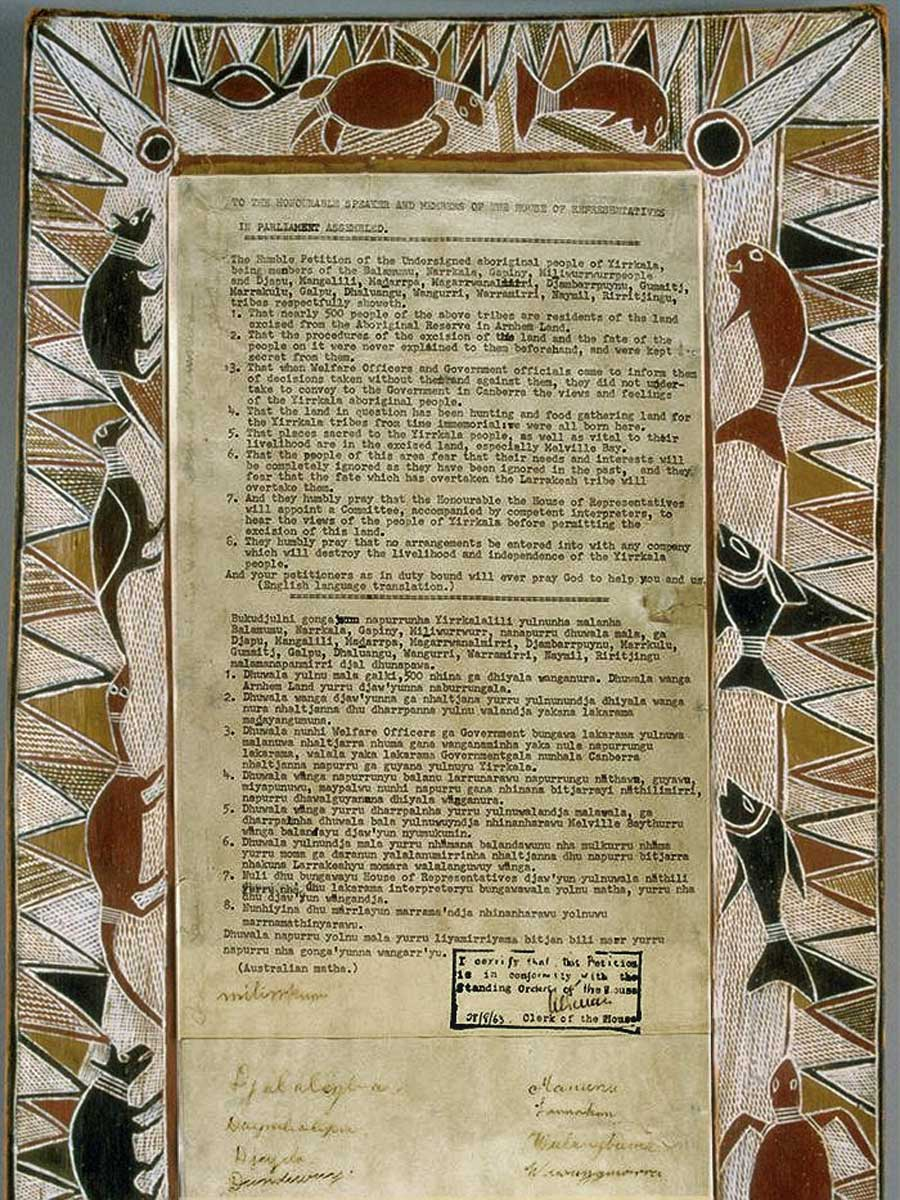
\includegraphics[width=\linewidth]{bark-petition.jpg}
    \caption[The Yirrkala Bark Petition]{
        The Yirrkala Bark Petition (1963) asks the Federal Government to
        reverse a mining lease granted on Yolngu land without their consent,
        and marks a key point in the Australian Land Rights movement.

        It is presented by text in English and in Yolngu Matha, with a
        painted border.  This is not decorative, but title deeds to the
        ancestoral estates of the signatories - showing how easy it can
        be to overlook or misunderstand Indigenous Knowledge.
        }
    \label{fig:bark-petition}
\end{wrapfigure}

The Yirrkala Bark Petition (\cref{fig:bark-petition}) provides a visible
example of how easy it can be for assumptions or misunderstandings to make
Indigenous knowledge or perspectives invisible.  The petition is presented
in English, and in Yolngu Matha (the shared language of the Yolngu people).
Few non-Indigenous readers realise that the border is not decorative: it is
also a legal document, recording the title deeds of the signatories' ancestral
estates and providing the legal foundation of their objection to the mining
lease.
%
EXPAND - note that knowing a little or expectations can `blind' you to
what's really happening; importance of openness and checking assumptions.



\section{Australian Indigenous Seasons}
\label{sec:aus-indig-seasons}
\todo{write this section}

Summarise, compare and contrast Indigenous seasons literature.
Indigenous knowledge of phenology stretches back millennia - and much is
encoded in the seasonal calendars and traditions.\\


Documenting indigenous calendars - see eg \textit{Man of All Seasons} \citep{davis1989},
the Indigenous Weather Knowledge project \citet{BOM-iwk},
or CSIRO's Tropical Rivers and Coastal Knowledge (TRaCK) program \citep{CSIROcals,oconnor2010}.


This section is not finished, but you get a pretty good idea where it's
going.  Mainly it needs to be fleshed out with examples, references, etc.

Indigenous seasonal calendars are qualitatively different to the European
system, which was marked by lunar and later solar cycles.  By contrast,
Australian indigenous seasonal calendars are defined by climatic and ecological
cycles, with all the sensitivity to local context and variation between years
that implies.

For practical use, a local and long-tested seasonal calendar is likely to have
substantial advantages over one imported from Europe - at least for
applications which depend on an understanding of Australia's environment, such
as fire or natural resource management.

European seasons are adapted for agriculture in temperate regions.

Australian Indigenous calendars are generally adapted to a hunter-gatherer,
more mobile lifestyle.  They also must cope with a far higher degree of
interannual variation and offer more complex detail to be as useful.  It's no
coincidence that the calendar is based directly on the important climate
variables and marked by ecological events:  instead of ``the Wet is usually a
good time for these foods'', the knowledge is more like ``after the first big
storm (which marks this season), all the fish gather in these places''.



\todo{survey the general and specific projects documenting Australian Indigenous
seasons, and comment on each.}

General - BOM-IWK, CSIRO TRaCK project, CDU?.  For Yolngu seasons, Davis, Atlas, and I.

\todo{Un-comment Tiwi Calendar; currently disabled due to large file size and slow rendering}
%\begin{landscape}
%\begin{figure}[p]
%    \centering
%    \includegraphics[width=\paperwidth]{TiwiSeasons.pdf}
%    \caption[The Tiwi Seasons Calendar \citep{CSIROcals}]{
%        The Tiwi Seasons Calendar \citep{CSIROcals}.
%        This calendar shows month of year in the outermost ring,
%        then three `major' Tiwi seasons recognised by weather.
%        Note that \textit{Kumunupunari} does not have a sharp boundary with \textit{Tiyari}!
%        Within this ring are smaller seasons, recognised by weather
%        or ecological events and associated with particular activities.
%        This format is designed for the circle to rotate, encouraging interaction or observation.
%        }
%    \label{fig:tiwi-seasons}
%\end{figure}
%\end{landscape}


\begin{figure}[h]
    \centering
    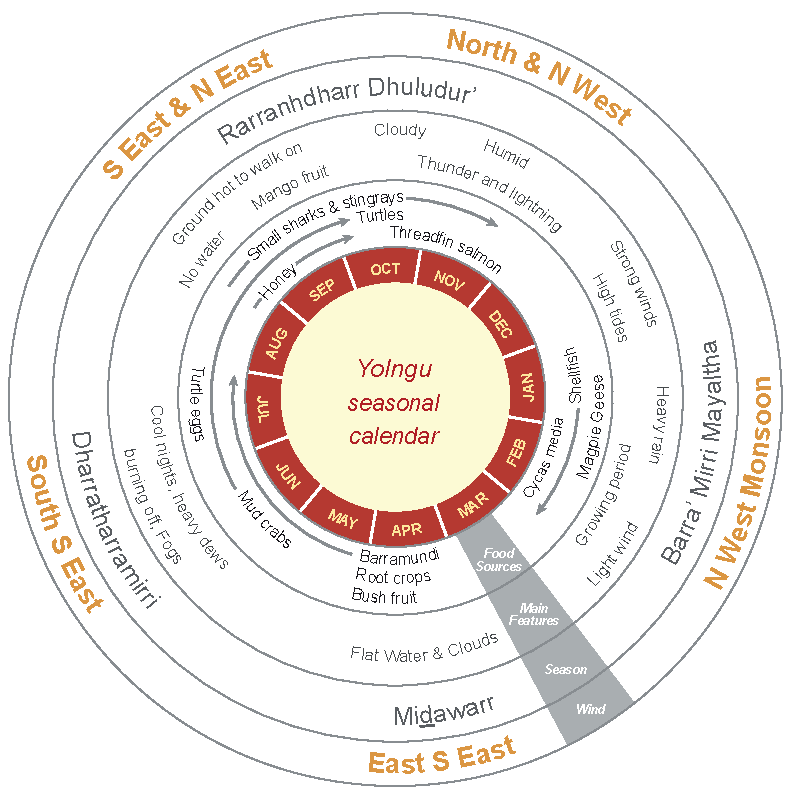
\includegraphics[width=0.7\textwidth]{davis1989_yolngu_seasons.pdf}
    \caption[Conceptual Yolngu seasonal calendar \citep{davis1989}]{
        Conceptual Yolngu seasonal calendar, redrawn from \citet[p2]{davis1989}.
        This calendar shows a glimpse of the relationships between season,
        prevailing wind, typical conditions, and available foods.
        It also shows typical gregorian months, for non-Indigenous readers.
        }
    \label{fig:yolngu-seasons}
\end{figure}




\subsection{The Gap in the Literature}

There is a paucity of research which treats indigenous knowledge
as a \emph{framework for} research, instead of an \emph{object of} research.
This gap in the literature persists despite the novely and potential value
of combining Indigenous seasonal knowledge with quantitative climate science.

After -detailed search strategy-, I was unable to identify any studies which
quantified indigenous Australian seasons.  PARA ON LIT SEARCH STRATEGY




\section{Methods}
\label{sec:lit-methods}
\todo{write this section}


\subsection{Research with Indigenous People}

VERY INCOMPLETE

Rather than structured interviews or a written survey, I conduct minimally-
directed conversations with research participants.  Bringing avoidable
paperwork to an indigenous community is generally not culturally appropriate,
as it can devolve into mutual frustration rather than mutual learning.  An
assumption of literacy may exclude potential participants where English is
often a fourth (or sixth, or later!) language.

Calendars and seasons are a topic which is not usually secret business, though
there may be particular sacred topics associated with them.  Especially with an
explicit invitation to come and learn, there is little risk of inappropriate
sharing of information.


Relationships are a key part of cross-cultural research.  See Sue Smith, as
Sean has mentioned.

This collaborative and cross-cultural approach has been and will be a
significant influence on the direction of the research. (explore it more then)



\subsection{Quantitative handling of seasons}

Some stuff will move here.  Eg Norway (iirc) winter detection,
references for various approaches to threshold detection,
impact of non-locally-monotonic trends, etc.

Historical climatology is important in that it informs my methods,
but also for the concept and to contextualise the research.  May lead to
some comparisons between `lay knowledge' and IEK (an important point).


There is a considerable body of literature dealing with seasons defined
by observed environmental change - from temperature thresholds in
Scandinavia to 'leaf out' for botanists or butterflies for zoologists.

While such definitions are highly dependent on context, some common
elements can be observed.

Monotonic changes and qualitative changes are easiest to pin down.
Ie binary states, and/or only passing the threshold once per year.

\todo{more on this, add references.}

I've started reading the literature on historical climatology, but don't have
enough depth to write much yet.  It's going to be an important angle though.

Matching oral history with numerical data is an established technique in
climate science, as recorded observations can greatly assist in reconstruction
of conditions before the instrumental record began.  In this case, observations
within living memory are an excellent source, as the instrumental record is
even today very sparse in Arnhem Land.  Investigation of social adaptation to
local climate is an interesting and often closely linked field.

Look more into non-observational records; as far as I know dendrology etc has
not been done much in the region; this is relevant as a missing alternative to
oral histories.
